\PassOptionsToPackage{unicode=true}{hyperref} % options for packages loaded elsewhere
\PassOptionsToPackage{hyphens}{url}
\documentclass[12pt,ignorenonframetext,aspectratio=169]{beamer}
\IfFileExists{pgfpages.sty}{\usepackage{pgfpages}}{}
\setbeamertemplate{caption}[numbered]
\setbeamertemplate{caption label separator}{: }
\setbeamercolor{caption name}{fg=normal text.fg}
\beamertemplatenavigationsymbolsempty
\usepackage{lmodern}
\usepackage{amssymb}
\usepackage{amsmath}
\usepackage{ifxetex,ifluatex}
\usepackage{fixltx2e} % provides \textsubscript
\ifnum 0\ifxetex 1\fi\ifluatex 1\fi=0 % if pdftex
  \usepackage[T1]{fontenc}
  \usepackage[utf8]{inputenc}
\else % if luatex or xelatex
  \ifxetex
    \usepackage{mathspec}
  \else
    \usepackage{fontspec}
\fi
\defaultfontfeatures{Ligatures=TeX,Scale=MatchLowercase}






%
\fi

  \usetheme[]{iqss}






% use upquote if available, for straight quotes in verbatim environments
\IfFileExists{upquote.sty}{\usepackage{upquote}}{}
% use microtype if available
\IfFileExists{microtype.sty}{%
  \usepackage{microtype}
  \UseMicrotypeSet[protrusion]{basicmath} % disable protrusion for tt fonts
}{}


\newif\ifbibliography


\hypersetup{
      pdftitle={Production relationships},
        pdfauthor={Deependra Dhakal},
          pdfborder={0 0 0},
    breaklinks=true}
%\urlstyle{same}  % Use monospace font for urls







% Prevent slide breaks in the middle of a paragraph:
\widowpenalties 1 10000
\raggedbottom

  \AtBeginPart{
    \let\insertpartnumber\relax
    \let\partname\relax
    \frame{\partpage}
  }
  \AtBeginSection{
    \ifbibliography
    \else
      \let\insertsectionnumber\relax
      \let\sectionname\relax
      \frame{\sectionpage}
    \fi
  }
  \AtBeginSubsection{
    \let\insertsubsectionnumber\relax
    \let\subsectionname\relax
    \frame{\subsectionpage}
  }



\setlength{\parindent}{0pt}
\setlength{\parskip}{6pt plus 2pt minus 1pt}
\setlength{\emergencystretch}{3em}  % prevent overfull lines
\providecommand{\tightlist}{%
  \setlength{\itemsep}{0pt}\setlength{\parskip}{0pt}}

  \setcounter{secnumdepth}{0}


  \usepackage{booktabs}
  \usepackage{longtable}
  \usepackage{emptypage}
  \usepackage{array}
  \usepackage{multirow}
  \usepackage{wrapfig}
  \usepackage{float}
  \usepackage{colortbl}
  \usepackage{pdflscape}
  \usepackage{tabu}
  \usepackage{threeparttable}
  \usepackage{threeparttablex}
  \usepackage[normalem]{ulem}
  \usepackage{rotating}
  \usepackage{makecell}
  \usepackage{xcolor}
  \usepackage{tikz} % required for image opacity change
  \usepackage[absolute,overlay]{textpos} % for text formatting


  % this font option is amenable for beamer
  \setbeamerfont{caption}{size=\tiny}


%% IQSS overrides
\iqsssectiontitle{Outline}

\AtBeginSection[]{
  \title{\insertsectionhead}
  {
    \definecolor{white}{rgb}{0.776,0.357,0.157}
    \definecolor{iqss@orange}{rgb}{1,1,1}
    \ifnum \insertmainframenumber > \insertframenumber
    \frame{
      \frametitle{\iqsssectiontitleheader}
      \tableofcontents[currentsection]
    }
    \else
    \frame{
      \frametitle{Backup Slides}
      \tableofcontents[sectionstyle=shaded/shaded,subsectionstyle=shaded/shaded/shaded]
    }
    \fi
  }
}

\AtBeginSubsection[]{}

%%


  \title[]{Production relationships}



  \author[
        Deependra Dhakal
    ]{Deependra Dhakal}

  \institute[
    ]{
    GAASC, Baitadi \and Tribhuwan University
    }

\date[
      \today
  ]{
      \today
        }

\begin{document}

% Hide progress bar and footline on titlepage
  \begin{frame}[plain]
  \titlepage
  \end{frame}



\hypertarget{introduction}{%
\section{Introduction}\label{introduction}}

\begin{frame}{Product relationships}
\protect\hypertarget{product-relationships}{}
\begin{itemize}
\tightlist
\item
  All major production relationships can be categorized under three
  categories. i.e.:

  \begin{enumerate}
  \tightlist
  \item
    Factor-product relationship
  \item
    Factor-factor relationship
  \item
    Product-product relationship
  \end{enumerate}
\end{itemize}
\end{frame}

\hypertarget{factor-product-relationship}{%
\section{Factor-product
relationship}\label{factor-product-relationship}}

\begin{frame}{Background}
\protect\hypertarget{background}{}
\begin{itemize}
\tightlist
\item
  When concerned with resource allocation for production optimization,
  an understanding of input-output or factor-product relationship is
  important.
\item
  First, study of physical or technical relationship is important.
  Second, for decision making, application of economic choice indicators
  such as price ratio is required.
\item
  In a simple scenario, we details the physical factor-product
  relationship of a single variable resoruce and single product.
\item
  Many time resources or capacities of technical units, such as a ropani
  of land or a cow, are fixed and choice is to vary the input of only
  one factor -- such as fertilizer \alertc{OR} labor.
\item
  Other inputs such as fixed capital, buildings, implements and
  technical knowhow remain the same.
\end{itemize}
\end{frame}

\begin{frame}{}
\protect\hypertarget{section}{}
\begin{itemize}
\tightlist
\item
  Under such situation question of how much of certain input (amount of
  fertilizer or feed to a cow) to apply arises ?
\item
  This situtation is dealt by single factor-product relationships. a.k.a
  single variable production function (in a production function various
  levels of input are involved with corresponding output of the
  product).
\end{itemize}

\begin{block}{Inputs have several different names:}
\protect\hypertarget{inputs-have-several-different-names}{}
Inputs = factors = factors of production = resources = A, L, K, M

\begin{quote}
\textbf{A}: Land (Natural and biological resources, climate.)
\newline \textbf{L}: Labor (Human resources.) \newline \textbf{K}:
Capital (Manufactured resources, which include buildings, machines,
tools, and equipment.) \newline \textbf{M}: Management (The
entrepreneur, or individual, who combines the other resources into
inputs.)
\end{quote}
\end{block}
\end{frame}

\begin{frame}{Example: Production function of wheat}
\protect\hypertarget{example-production-function-of-wheat}{}
To isolate the relationship between nitrogen and wheat yields, the
agronomists (or other biophysical scientists) will hold constant all
inputs other than the one that they are isolating, in this case
nitrogen.

\[Y = f(N | L, K, M, A)\]

This relationship is highly important, since too little nitrogen means
the yields will be lower than the potential, and too much nitrogen will
``burn'' the crop, causing smaller yields. Figure
\ref{fig:nitrogen-wheat} shows the connection between nitrogen
applications and wheat yields.
\end{frame}

\begin{frame}{}
\protect\hypertarget{section-1}{}
\begin{figure}
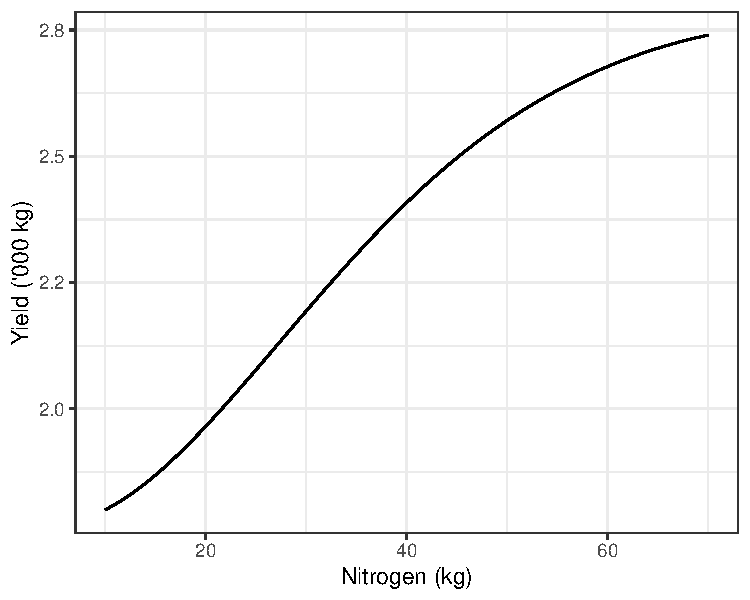
\includegraphics[width=0.5\linewidth]{production_relationship_files/figure-beamer/nitrogen-wheat-1} \caption{Relationship between nitrogen application and yield}\label{fig:nitrogen-wheat}
\end{figure}
\end{frame}

\begin{frame}{Concept of optimum production}
\protect\hypertarget{concept-of-optimum-production}{}
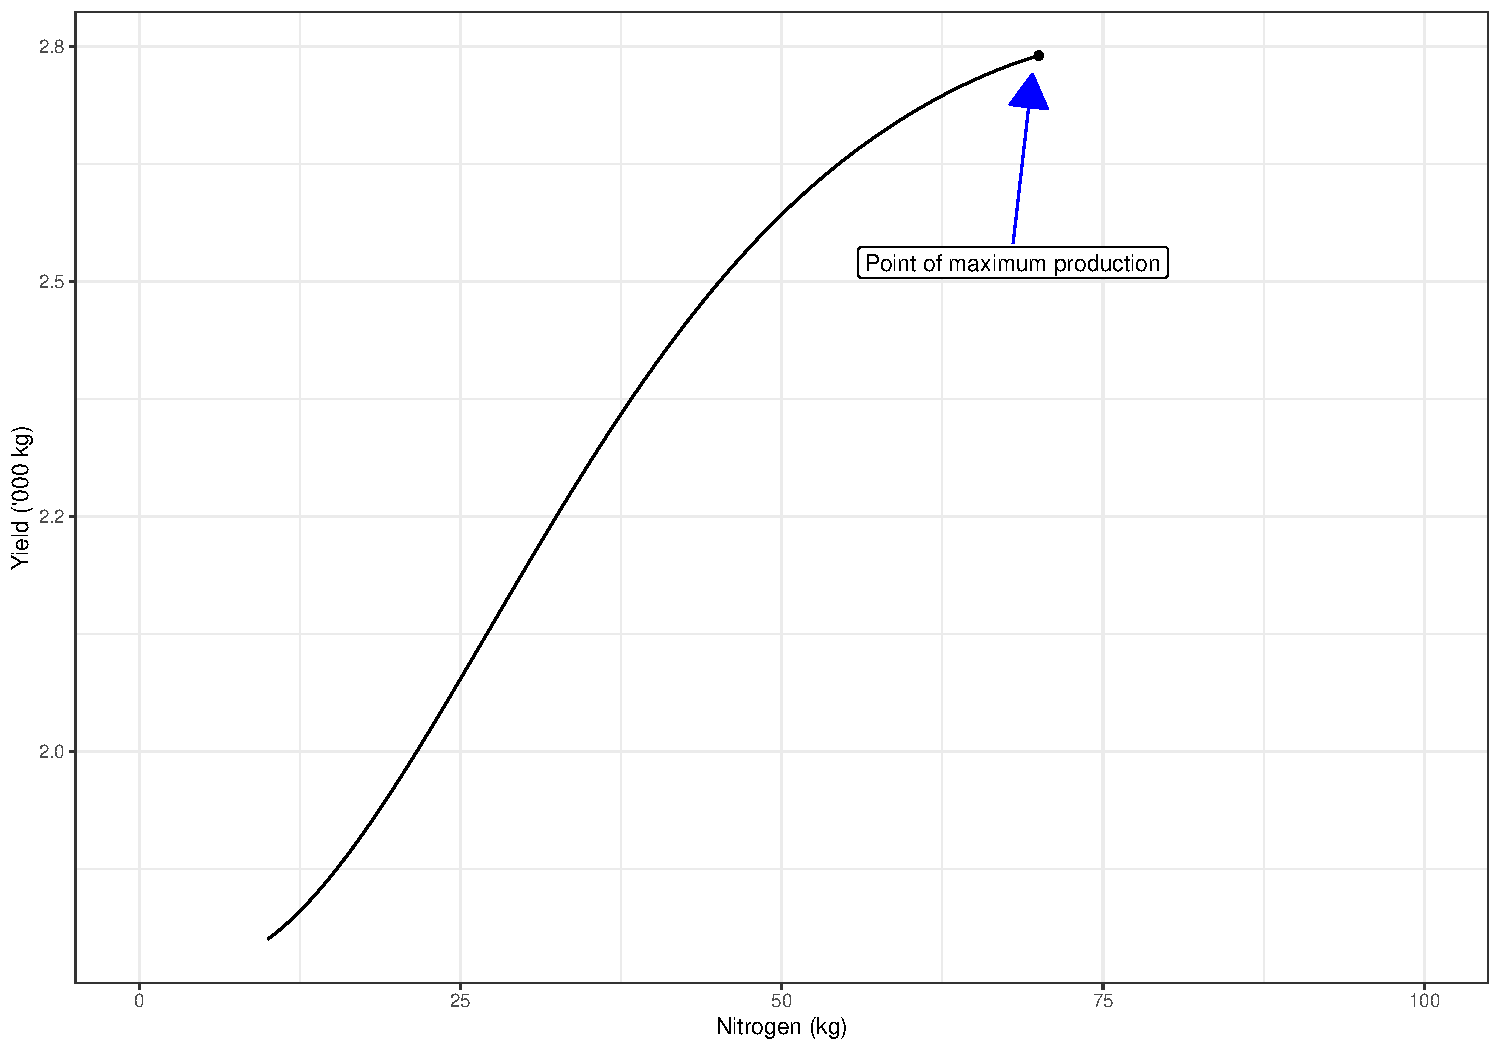
\includegraphics[width=0.45\linewidth]{production_relationship_files/figure-beamer/nitrogen-wheat-optimum-production-1}

\begin{itemize}
\tightlist
\item
  The point of maximum physical wheat yield (N*) is not always the
  optimal economic wheat yield. This is because nitrogen is a scarce
  resource, and costs money to purchase. In fact, fertilizer is one of
  the major costs of production for farmers in most agricultural
  regions.
\end{itemize}
\end{frame}

\begin{frame}{}
\protect\hypertarget{section-2}{}
\begin{itemize}
\tightlist
\item
  If nitrogen were free, then the optimal application to a wheat field
  would always be N* in Figure \ref{fig:nitrogen-wheat}, since this is
  the level of nitrogen that maximizes production.
\item
  However, since it costs money to purchase and use fertilizer, the
  farmer will stop applying it at a point to the left of N*. Finding the
  optimal amount of nitrogen to apply requires application of economic
  principles. Economic reasoning will help determine the exact point
  where the benefits of using N minus the costs are maximized.
\item
  Producers will not maximize production, because it costs too much.
  Instead, they will maximize profits.
\end{itemize}
\end{frame}

\begin{frame}{Types of production functions}
\protect\hypertarget{types-of-production-functions}{}
\begin{itemize}
\tightlist
\item
  There can be three types of input-output relationships in the
  production of a commodity where one input is varied and the quantities
  of all other inputs are fixed.

  \begin{enumerate}
  \tightlist
  \item
    Constant marginal rate of returns (Constant productivity)
  \item
    Increasing marginal rate of returns (Increasing productivity)
  \item
    Decreasing marginal rate of returns (Decreasing productivity)
  \end{enumerate}
\end{itemize}
\end{frame}

\begin{frame}{Contant marginal rate of returns}
\protect\hypertarget{contant-marginal-rate-of-returns}{}
\begin{itemize}
\tightlist
\item
  Each additional unit of the variable input when applied to fixed
  factors, produces an equal amount of additional product. The amount of
  product increases by the same magnitude for each additional unit of
  input.
\item
  Not a very common relationship in agriculture and holds true only for
  limited range.
\item
  Example:

  \begin{enumerate}
  \tightlist
  \item
    Addition of one acre of land (technology and other factors being
    same) will add the same amount of product.
  \item
    An addition of one tractor plus driver will do the same amount of
    work as previous tractor driver unit did.
  \end{enumerate}
\end{itemize}
\end{frame}

\begin{frame}{}
\protect\hypertarget{section-3}{}
\begin{figure}
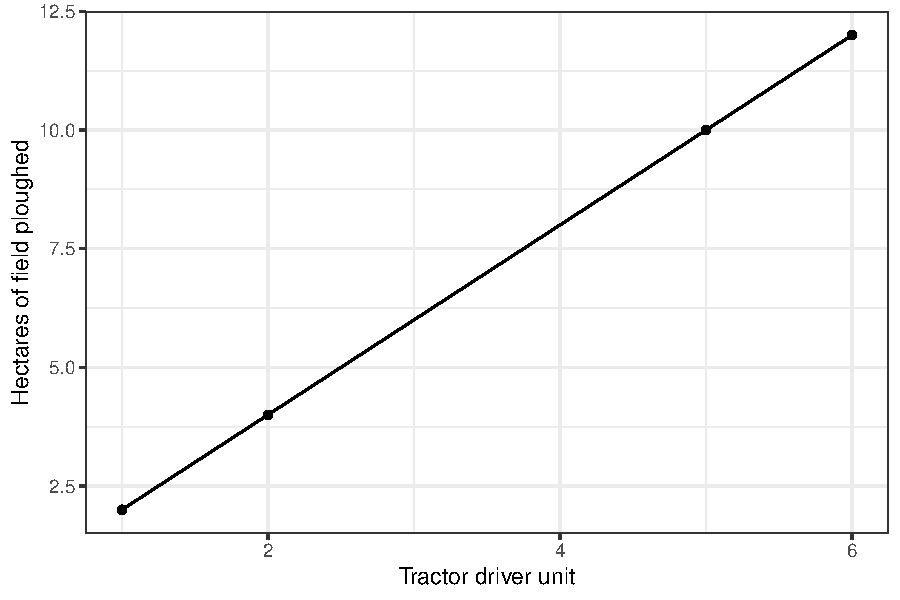
\includegraphics[width=0.45\linewidth]{production_relationship_files/figure-beamer/tractor-driver-unit-cmr-fig-1} \caption{Constant marginal rate of returns for a input-output relationship between number of tractor plus driver unit recruits and hectares of land ploughed.}\label{fig:tractor-driver-unit-cmr-fig}
\end{figure}
\end{frame}

\begin{frame}{}
\protect\hypertarget{section-4}{}
\begin{table}

\caption{\label{tab:tractor-driver-unit-cmr-tab}Constant marginal rate of returns for a input-output relationship between number of tractor plus driver unit recruits and hectares of land ploughed.}
\centering
\fontsize{6}{8}\selectfont
\begin{tabular}[t]{rrrrr}
\toprule
tractor driver unit & field ploughed & marginal tractor driver unit & marginal field ploughed & marginal rate returns\\
\midrule
1 & 2 &  &  & 2\\
2 & 4 & 1 & 2 & 2\\
5 & 10 & 3 & 6 & 2\\
6 & 12 & 1 & 2 & 2\\
\bottomrule
\end{tabular}
\end{table}
\end{frame}

\begin{frame}{Increasing marginal rate of returns}
\protect\hypertarget{increasing-marginal-rate-of-returns}{}
\begin{itemize}
\tightlist
\item
  Every additional or marginal unit of input adds more to the total
  product than the previous unit, i.e., addition to total product is at
  an increasing rate.
\item
  In actual practice, the cases of purely increasing returns are rarely
  available except, again, in very limited range.
\item
  This relationship is possible when the fixed factors of production are
  in excess capacity and addition of the small units of a variable
  resource makes more and more efficient use of fixed resources.
\item
  Example:

  \begin{enumerate}
  \tightlist
  \item
    Small quanity of wheat seed applied when other factors of production
    such as fertilizer, irrigation and other cultural practices can be
    used at high levels will give low returns.
  \end{enumerate}
\end{itemize}
\end{frame}

\begin{frame}{}
\protect\hypertarget{section-5}{}
\begin{figure}
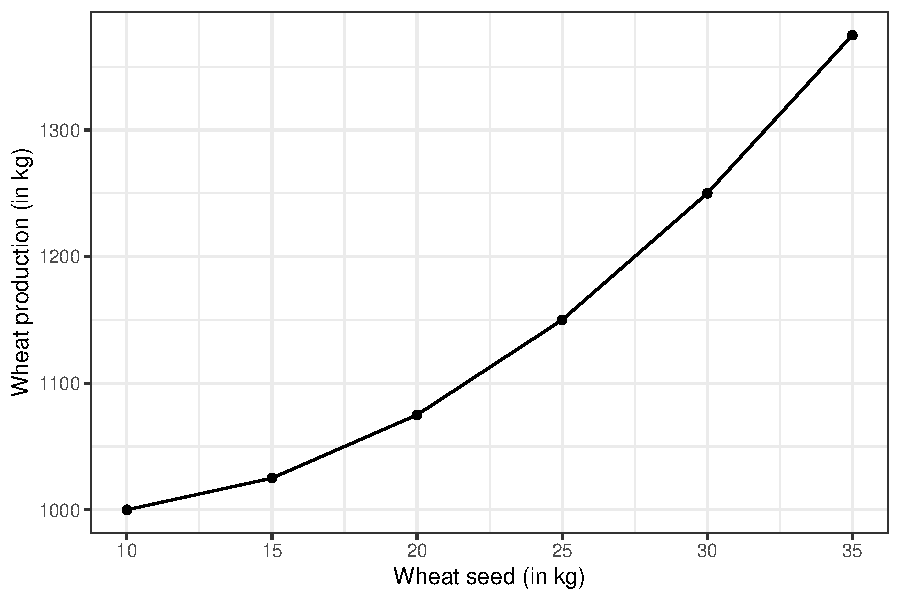
\includegraphics[width=0.45\linewidth]{production_relationship_files/figure-beamer/nitrogen-wheat-imr-fig-1} \caption{Increasing marginal rate of returns for hypothetical wheat production scenario.}\label{fig:nitrogen-wheat-imr-fig}
\end{figure}
\end{frame}

\begin{frame}{}
\protect\hypertarget{section-6}{}
\begin{table}

\caption{\label{tab:nitrogen-wheat-imr-tab}Increasing marginal rate of return for hypothetical wheat production scenario.}
\centering
\fontsize{6}{8}\selectfont
\begin{tabular}[t]{rrrrr}
\toprule
wheat seed & marginal wheat seed & wheat production & marginal wheat production & marginal rate returns\\
\midrule
10 &  & 1000 &  & \\
15 & 5 & 1025 & 25 & 5\\
20 & 5 & 1075 & 50 & 10\\
25 & 5 & 1150 & 75 & 15\\
30 & 5 & 1250 & 100 & 20\\
\addlinespace
35 & 5 & 1375 & 125 & 25\\
\bottomrule
\end{tabular}
\end{table}
\end{frame}

\hypertarget{bibliography}{%
\section{Bibliography}\label{bibliography}}

\begin{frame}{For more information}
\protect\hypertarget{for-more-information}{}
\end{frame}




\end{document}
